\documentclass[border=2pt,tikz]{standalone}
\usepackage[T1]{fontenc}
% Nature Portfolio / Scientific Data shared TikZ style for IRexp figures.
% Width: 183 mm double-column. Typography: Helvetica-class (phv).
\RequirePackage{tikz}
\RequirePackage{pgfplots}
\RequirePackage{xcolor}
\RequirePackage{helvet}
\IfFileExists{sansmathfonts.sty}{\RequirePackage{sansmathfonts}}{}
\renewcommand{\familydefault}{\sfdefault}
\pgfplotsset{compat=1.18}
\usetikzlibrary{
  arrows.meta,calc,positioning,fit,shapes.geometric,shapes.misc,
  backgrounds,shadows.blur,patterns,decorations.pathreplacing
}

% ---- Paul Tol / NMRexp-matched palette ----
\definecolor{nmrBlue}{HTML}{4A7EBB}
\definecolor{nmrBlueDark}{HTML}{2E5F8F}
\definecolor{nmrBlueLight}{HTML}{A8C8E8}
\definecolor{nmrPeach}{HTML}{E8B48C}
\definecolor{nmrNavy}{HTML}{1B3D5C}
\definecolor{nmrRed}{HTML}{C44E52}
\definecolor{nmrGreen}{HTML}{3D8B5E}
\definecolor{nmrOrange}{HTML}{D97B32}
\definecolor{ink}{HTML}{1A1A1A}
\definecolor{muted}{HTML}{7A7F85}
\definecolor{note}{HTML}{5C636A}
\definecolor{faint}{HTML}{E8EAEC}
\definecolor{ghost}{HTML}{C5C9CD}
\definecolor{tintBlue}{HTML}{EEF3F8}
\definecolor{tintGreen}{HTML}{EAF4EE}

\newcommand{\NatureFont}{\fontfamily{phv}\selectfont}
\newcommand{\PanelLabel}[1]{%
  {\NatureFont\bfseries\fontsize{8}{9.6}\selectfont #1}%
}
\newcommand{\FigBody}{\NatureFont\fontsize{7}{8.4}\selectfont}
\newcommand{\FigSmall}{\NatureFont\fontsize{5.5}{6.6}\selectfont}
\newcommand{\FigAxis}{\NatureFont\fontsize{7}{8.4}\selectfont}

\tikzset{
  nature arrow/.style={
    -{Latex[length=1.6mm,width=1.3mm]},
    line width=0.55pt, ink
  },
  nature arrow grey/.style={
    -{Latex[length=1.6mm,width=1.3mm]},
    line width=0.5pt, note
  },
  stage card/.style={
    draw=nmrBlueDark, line width=0.7pt, rounded corners=2.2pt,
    fill=white, inner sep=3pt, align=center, font=\FigBody
  },
  stage header/.style={
    fill=nmrBlueDark, text=white, font=\FigBody\bfseries,
    rounded corners=2.2pt, inner sep=2.5pt, align=center
  },
  soft card/.style={
    draw=ghost, line width=0.55pt, rounded corners=2.2pt,
    fill=white, inner sep=3.5pt, align=left, font=\FigBody
  },
}

\pgfplotsset{
  nature axis/.style={
    tick label style={font=\FigSmall, /pgf/number format/assume math mode},
    label style={font=\FigAxis\bfseries},
    title style={font=\FigBody\bfseries, color=ink},
    axis line style={ink, line width=0.5pt},
    tick style={ink, line width=0.45pt},
    major grid style={faint, line width=0.35pt},
    axis x line=bottom,
    axis y line=left,
    enlarge x limits=false,
    clip=false,
  },
  nature hbar/.style={
    nature axis,
    xbar,
    bar width=7pt,
    y=data,
    nodes near coords,
    every node near coord/.append style={
      font=\FigSmall, ink, anchor=west, /pgf/number format/fixed,
      /pgf/number format/1000 sep={,}
    },
    xtick=\empty,
    axis x line=none,
    y axis line style={ink, line width=0.55pt},
    ytick style={draw=none},
    y tick label style={font=\FigBody, ink, anchor=east},
    grid=major x,
    xmin=0,
  },
}

% Auto-generated from frozen_plot_data.json — do not edit by hand.
\newcommand{\IRexpTotal}{121233}
\newcommand{\IRexpStruct}{43060}
\newcommand{\IRexpCommercial}{88545}
\newcommand{\IRexpNMR}{87075}
\newcommand{\IRexpPMC}{119345}
\newcommand{\IRexpChemotion}{1888}
\newcommand{\IRexpNC}{21823}
\newcommand{\IRexpEmpty}{8963}
\newcommand{\IRexpSA}{1897}
\newcommand{\IRexpOther}{5}
\newcommand{\IRexpQuad}{33201}
\newcommand{\NMRexpN}{3370987}
\newcommand{\SDBSN}{54100}
\newcommand{\NISTN}{17000}
\newcommand{\BandMedian}{9}
\newcommand{\TxMAE}{0.0049}
\newcommand{\BandRecallPool}{0.9903}
\newcommand{\ListMatchPool}{0.9848}
\newcommand{\FailRate}{0.0321}

% Band histogram coordinates (x,y)
\newcommand{\BandHistCoords}{
(4,24556)
(6,22989)
(8,18726)
(10,14534)
(12,9959)
(14,7368)
(16,5241)
(18,3899)
(20,3017)
(22,2202)
(24,1822)
(26,1426)
(28,1069)
(30,826)
(32,698)
(34,534)
(36,386)
(38,408)
(40,298)
(42,250)
}

% Element bars
\newcommand{\ElementCommonCoords}{
(43047,8)% C
(38870,7)% O
(36292,6)% N
(12258,5)% S
(5939,4)% F
(7675,3)% Cl
(3923,2)% Br
(959,1)% Si
(859,0)% P
}
\newcommand{\ElementRareCoords}{
(904,8)% I
(270,7)% B
(384,6)% Se
(119,5)% Fe
(73,4)% Te
(64,3)% Sn
(1,2)% Ge
(16,1)% Na
(24,0)% K
}
\newcommand{\ElementCommonLabels}{C,O,N,S,F,Cl,Br,Si,P}
\newcommand{\ElementRareLabels}{I,B,Se,Fe,Te,Sn,Ge,Na,K}
\newcommand{\ElC}{43047}
\newcommand{\ElO}{38870}
\newcommand{\ElN}{36292}
\newcommand{\ElS}{12258}
\newcommand{\ElF}{5939}
\newcommand{\ElCl}{7675}
\newcommand{\ElBr}{3923}
\newcommand{\ElSi}{959}
\newcommand{\ElP}{859}
\newcommand{\ElI}{904}
\newcommand{\ElB}{270}
\newcommand{\ElSe}{384}
\newcommand{\ElFe}{119}
\newcommand{\ElTe}{73}
\newcommand{\ElSn}{64}
\newcommand{\ElGe}{1}
\newcommand{\ElNa}{16}
\newcommand{\ElK}{24}
\newcommand{\TxErrMedian}{0.0}
\newcommand{\TxErrCoords}{
(0.0250,196)
(0.0750,0)
(0.1250,0)
(0.1750,0)
(0.2250,0)
(0.2750,0)
(0.3250,0)
(0.3750,0)
(0.4250,1)
(0.4750,0)
(0.5250,1)
(0.5750,1)
(0.6250,0)
(0.6750,0)
(0.7250,0)
(0.7750,1)
(0.8250,0)
(0.8750,0)
(0.9250,0)
(0.9750,0)
(1.0250,0)
}
\newcommand{\TxErrBinWidth}{0.05000}
\newcommand{\PaperRecallMedian}{1.0}
\newcommand{\PaperRecallCoords}{
(0.0250,3)
(0.0750,0)
(0.1250,0)
(0.1750,0)
(0.2250,0)
(0.2750,0)
(0.3250,0)
(0.3750,0)
(0.4250,1)
(0.4750,0)
(0.5250,0)
(0.5750,0)
(0.6250,0)
(0.6750,0)
(0.7250,0)
(0.7750,0)
(0.8250,0)
(0.8750,1)
(0.9250,0)
(0.9750,0)
(1.0250,115)
}
\newcommand{\PaperRecallBinWidth}{0.05000}
\newcommand{\ListMatchMedian}{1.0}
\newcommand{\ListMatchCoords}{
(0.0250,4)
(0.0750,0)
(0.1250,0)
(0.1750,0)
(0.2250,0)
(0.2750,0)
(0.3250,0)
(0.3750,0)
(0.4250,0)
(0.4750,0)
(0.5250,1)
(0.5750,0)
(0.6250,2)
(0.6750,1)
(0.7250,1)
(0.7750,0)
(0.8250,1)
(0.8750,0)
(0.9250,0)
(0.9750,0)
(1.0250,109)
}
\newcommand{\ListMatchBinWidth}{0.05000}
\newcommand{\FailCtMedian}{0.0}
\newcommand{\FailCtCoords}{
(0.1250,271)
(0.3750,0)
(0.6250,0)
(0.8750,0)
(1.1250,9)
(1.3750,0)
(1.6250,0)
(1.8750,0)
(2.1250,0)
(2.3750,0)
}
\newcommand{\FailCtBinWidth}{0.25000}


\begin{document}
\NatureFont
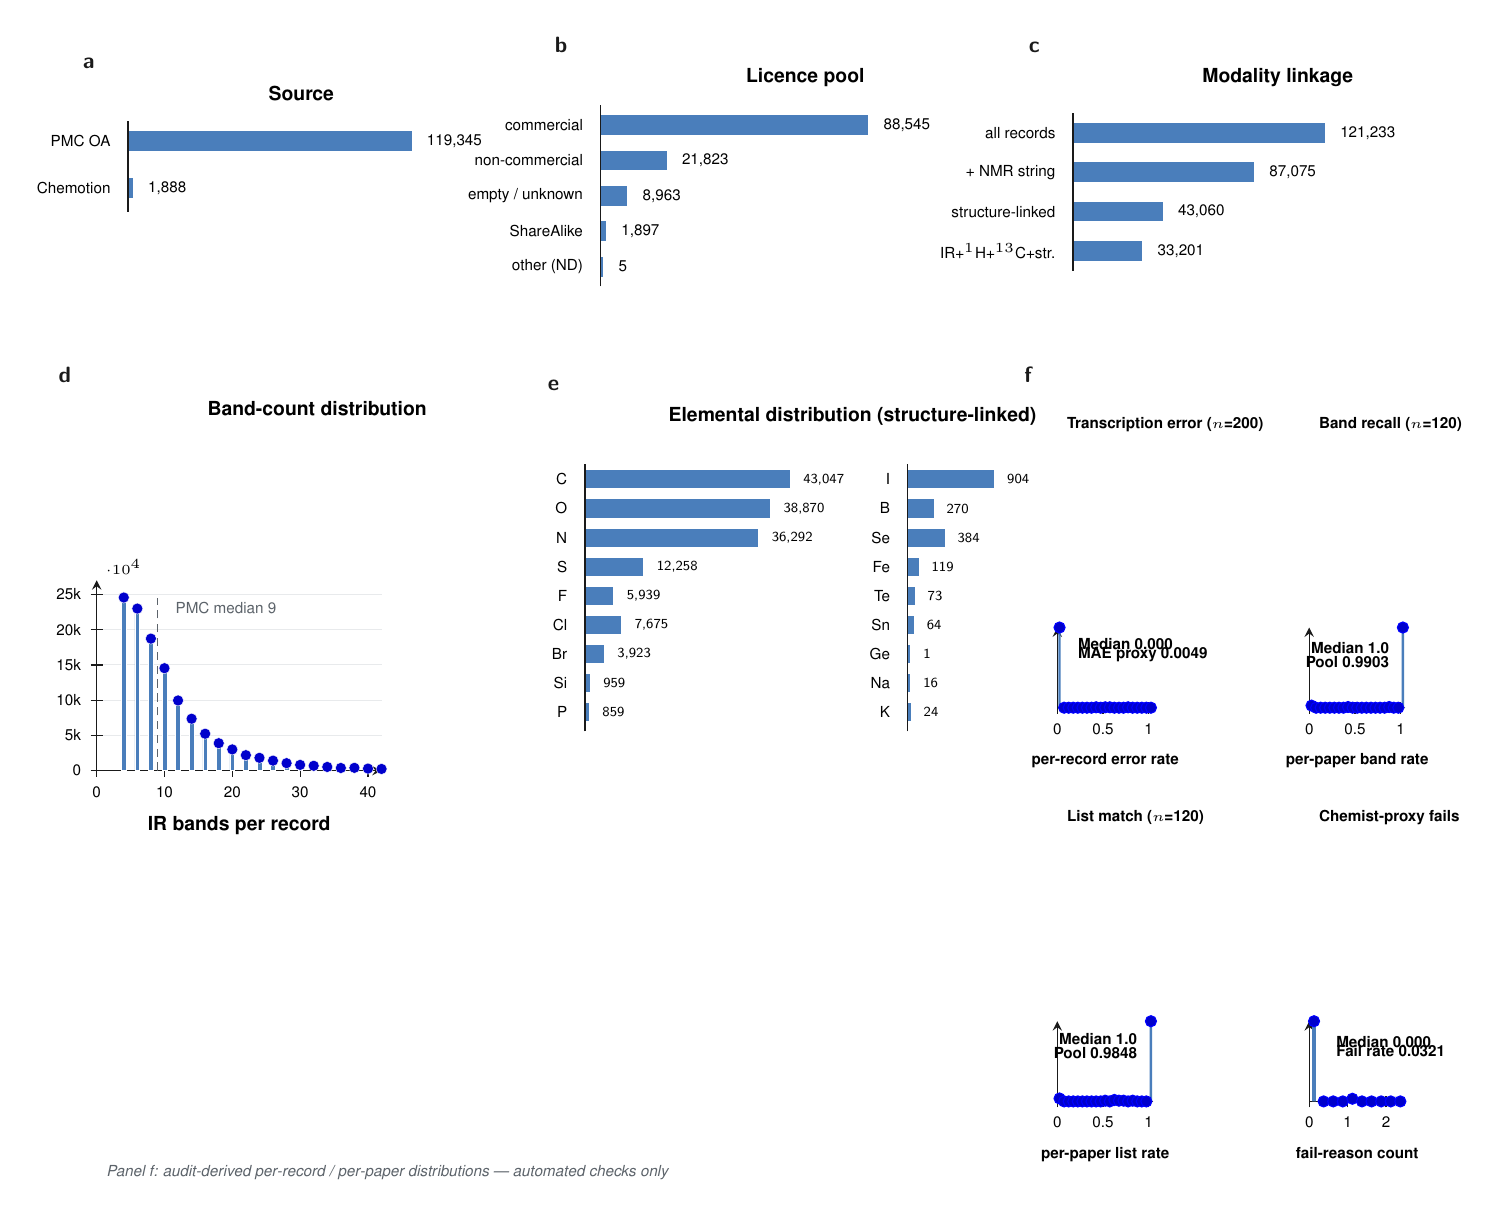
\begin{tikzpicture}[x=1mm,y=1mm]

\newcommand{\plabel}[2]{\node[font=\fontsize{8}{9.6}\selectfont\bfseries,ink,anchor=south east] at (#1) {#2};}
\newcommand{\hbarrow}[5]{% y, label, width_mm, value_text, label_x
  \node[anchor=east,font=\FigSmall] at (#5,#1) {#2};
  \fill[nmrBlue] (0,#1-1.25) rectangle (#3,#1+1.25);
  \node[anchor=west,font=\FigSmall] at (#3+0.7,#1) {#4};
}

% ---- a Source ----
\begin{scope}[shift={(12,122)}]
  \plabel{-3,18}{a}
  \node[font=\FigBody\bfseries] at (22,16) {Source};
  \hbarrow{10}{PMC OA}{36}{119{,}345}{-1}
  \hbarrow{4}{Chemotion}{0.6}{1{,}888}{-1}
  \draw[ink,line width=0.55pt] (0,1) -- (0,12.5);
\end{scope}

% ---- b Licence ----
\begin{scope}[shift={(72,116)}]
  \plabel{-3,26}{b}
  \node[font=\FigBody\bfseries] at (26,24) {Licence pool};
  \hbarrow{18}{commercial}{34}{88{,}545}{-1}
  \hbarrow{13.5}{non-commercial}{8.4}{21{,}823}{-1}
  \hbarrow{9}{empty / unknown}{3.4}{8{,}963}{-1}
  \hbarrow{4.5}{ShareAlike}{0.7}{1{,}897}{-1}
  \hbarrow{0}{other (ND)}{0.35}{5}{-1}
  \draw[ink,line width=0.55pt] (0,-2.5) -- (0,20.5);
\end{scope}

% ---- c Modality ----
\begin{scope}[shift={(132,118)}]
  \plabel{-3,24}{c}
  \node[font=\FigBody\bfseries] at (26,22) {Modality linkage};
  \hbarrow{15}{all records}{32}{121{,}233}{-1}
  \hbarrow{10}{+ NMR string}{23.0}{87{,}075}{-1}
  \hbarrow{5}{structure-linked}{11.4}{43{,}060}{-1}
  \hbarrow{0}{IR+$^{1}$H+$^{13}$C+str.}{8.8}{33{,}201}{-1}
  \draw[ink,line width=0.55pt] (0,-2.5) -- (0,17.5);
\end{scope}

% ---- d Band hist ----
\begin{scope}[shift={(8,52)}]
  \plabel{-2,48}{d}
  \node[font=\FigBody\bfseries] at (28,46) {Band-count distribution};
  \begin{axis}[
    nature axis,
    at={(0mm,0mm)}, anchor=south west,
    width=52mm, height=40mm,
    ymin=0, ymax=27000, xmin=0, xmax=42,
    xlabel={IR bands per record},
    xlabel style={font=\FigAxis\bfseries},
    ytick={0,5000,10000,15000,20000,25000},
    yticklabels={0,5k,10k,15k,20k,25k},
    ymajorgrids=true,
    tick label style={font=\FigSmall},
  ]
  \addplot+[ybar, bar width=1.7pt, fill=nmrBlue, draw=white, line width=0.15pt, forget plot]
    coordinates {\BandHistCoords};
  \draw[note, line width=0.55pt, densely dashed]
    (axis cs:\BandMedian,0) -- (axis cs:\BandMedian,24500);
  \node[font=\FigSmall,note,anchor=west] at (axis cs:10.2,23000) {PMC median 9};
  \end{axis}
\end{scope}

% ---- e Elements ----
\begin{scope}[shift={(70,55)}]
  \plabel{-2,44}{e}
  \node[font=\FigBody\bfseries] at (34,42) {Elemental distribution (structure-linked)};
  \foreach \i/\sym/\ww/\txt in {%
    0/C/26.0/43{,}047,%
    1/O/23.5/38{,}870,%
    2/N/22.0/36{,}292,%
    3/S/7.4/12{,}258,%
    4/F/3.6/5{,}939,%
    5/Cl/4.6/7{,}675,%
    6/Br/2.4/3{,}923,%
    7/Si/0.6/959,%
    8/P/0.5/859%
  } {
    \pgfmathsetmacro{\yy}{34-\i*3.7}
    \node[anchor=east,font=\FigSmall] at (-1,\yy) {\sym};
    \fill[nmrBlue] (0,{\yy-1.15}) rectangle (\ww,{\yy+1.15});
    \node[anchor=west,font=\fontsize{4.8}{5.5}\selectfont] at ({\ww+0.5},\yy) {\txt};
  }
  \draw[ink,line width=0.55pt] (0,2) -- (0,36);
  \foreach \i/\sym/\ww/\txt in {%
    0/I/11.0/904,%
    1/B/3.3/270,%
    2/Se/4.7/384,%
    3/Fe/1.4/119,%
    4/Te/0.9/73,%
    5/Sn/0.8/64,%
    6/Ge/0.35/1,%
    7/Na/0.35/16,%
    8/K/0.4/24%
  } {
    \pgfmathsetmacro{\yy}{34-\i*3.7}
    \node[anchor=east,font=\FigSmall] at (40,\yy) {\sym};
    \fill[nmrBlue] (41,{\yy-1.15}) rectangle ({41+\ww},{\yy+1.15});
    \node[anchor=west,font=\fontsize{4.8}{5.5}\selectfont] at ({41+\ww+0.4},\yy) {\txt};
  }
  \draw[ink,line width=0.55pt] (41,2) -- (41,36);
\end{scope}

% ---- f validation ----
\begin{scope}[shift={(130,8)}]
  \plabel{-2,92}{f}
  \begin{scope}[shift={(0,52)}]
    \node[font=\FigSmall\bfseries,anchor=west] at (0,36) {Transcription error ($n$=200)};
    \begin{axis}[nature axis,width=28mm,height=26mm,at={(0mm,0mm)},anchor=south west,
      xmin=0,xmax=1.05,ymin=0,xlabel={per-record error rate},
      xlabel style={font=\FigSmall\bfseries},ytick=\empty,
      tick label style={font=\FigSmall}]
      \addplot+[ybar,bar width=0.85pt,fill=nmrBlue,draw=none,forget plot] coordinates {\TxErrCoords};
      \node[font=\FigSmall\bfseries,anchor=west] at (axis cs:0.12,155) {Median 0.000};
      \node[font=\FigSmall\bfseries,anchor=west] at (axis cs:0.12,130) {MAE proxy \TxMAE};
    \end{axis}
  \end{scope}
  \begin{scope}[shift={(32,52)}]
    \node[font=\FigSmall\bfseries,anchor=west] at (0,36) {Band recall ($n$=120)};
    \begin{axis}[nature axis,width=28mm,height=26mm,at={(0mm,0mm)},anchor=south west,
      xmin=0,xmax=1.05,ymin=0,xlabel={per-paper band rate},
      xlabel style={font=\FigSmall\bfseries},ytick=\empty,
      tick label style={font=\FigSmall}]
      \addplot+[ybar,bar width=0.85pt,fill=nmrBlue,draw=none,forget plot] coordinates {\PaperRecallCoords};
      \node[font=\FigSmall\bfseries,anchor=east] at (axis cs:0.98,85) {Median 1.0};
      \node[font=\FigSmall\bfseries,anchor=east] at (axis cs:0.98,65) {Pool \BandRecallPool};
    \end{axis}
  \end{scope}
  \begin{scope}[shift={(0,2)}]
    \node[font=\FigSmall\bfseries,anchor=west] at (0,36) {List match ($n$=120)};
    \begin{axis}[nature axis,width=28mm,height=26mm,at={(0mm,0mm)},anchor=south west,
      xmin=0,xmax=1.05,ymin=0,xlabel={per-paper list rate},
      xlabel style={font=\FigSmall\bfseries},ytick=\empty,
      tick label style={font=\FigSmall}]
      \addplot+[ybar,bar width=0.85pt,fill=nmrBlue,draw=none,forget plot] coordinates {\ListMatchCoords};
      \node[font=\FigSmall\bfseries,anchor=east] at (axis cs:0.98,85) {Median 1.0};
      \node[font=\FigSmall\bfseries,anchor=east] at (axis cs:0.98,65) {Pool \ListMatchPool};
    \end{axis}
  \end{scope}
  \begin{scope}[shift={(32,2)}]
    \node[font=\FigSmall\bfseries,anchor=west] at (0,36) {Chemist-proxy fails};
    \begin{axis}[nature axis,width=28mm,height=26mm,at={(0mm,0mm)},anchor=south west,
      xmin=0,xmax=2.5,ymin=0,xlabel={fail-reason count},
      xlabel style={font=\FigSmall\bfseries},ytick=\empty,
      tick label style={font=\FigSmall}]
      \addplot+[ybar,bar width=1.3pt,fill=nmrBlue,draw=none,forget plot] coordinates {\FailCtCoords};
      \node[font=\FigSmall\bfseries,anchor=west] at (axis cs:0.45,200) {Median 0.000};
      \node[font=\FigSmall\bfseries,anchor=west] at (axis cs:0.45,170) {Fail rate \FailRate};
    \end{axis}
  \end{scope}
\end{scope}

\node[font=\FigSmall\itshape,note,anchor=west] at (8,1)
  {Panel f: audit-derived per-record / per-paper distributions --- automated checks only};

\end{tikzpicture}
\end{document}
